\documentclass[12pt,a4paper]{article}

% Paquetes esenciales para tipografía y formato académico
\usepackage[utf8]{inputenc}
\usepackage[T1]{fontenc}
\usepackage{lmodern} % Tipografía Latin Modern - alta legibilidad
\usepackage{microtype} % Mejoras tipográficas finas
\usepackage{geometry} % Control de márgenes
\usepackage{setspace} % Control de interlineado
\usepackage{graphicx} % Para imágenes
\usepackage{float} % Control de posición de figuras
\usepackage{caption} % Mejoras en captions
\usepackage{subcaption} % Subfiguras
\usepackage{booktabs} % Tablas profesionales
\usepackage{array} % Mejoras en tablas
\usepackage{multirow} % Celdas múltiples en tablas
\usepackage{tabularx} % Tablas con ancho ajustable
\usepackage{longtable} % Tablas multipágina
\usepackage{adjustbox} % Ajuste de cajas y tablas
\usepackage{xcolor} % Colores
\usepackage{hyperref} % Enlaces y PDF interactivo
\usepackage{amsmath} % Para fórmulas matemáticas
\usepackage{amssymb} % Símbolos matemáticos
\usepackage{fancyhdr} % Encabezados y pies de página
\usepackage{enumitem} % Listas mejoradas
\usepackage{titlesec} % Títulos personalizados

% Configuración de márgenes optimizada para formato académico
\geometry{
    a4paper,
    left=2.5cm,      % Margen izquierdo estándar académico
    right=2.5cm,     % Margen derecho
    top=2.5cm,       % Margen superior
    bottom=2.5cm,    % Margen inferior
    headheight=15pt,
    headsep=20pt,
    footskip=30pt
}

% Configuración de interlineado para mejor legibilidad
\renewcommand{\baselinestretch}{1.3} % 1.3 de interlineado (estándar académico)

% Configuración de colores para alto contraste
\definecolor{darkblue}{RGB}{0,51,102}
\definecolor{lightgray}{RGB}{245,245,245}

% Configuración de hyperref para accesibilidad
\hypersetup{
    colorlinks=true,
    linkcolor=darkblue,
    filecolor=darkblue,
    urlcolor=darkblue,
    citecolor=darkblue,
    bookmarks=true,
    bookmarksopen=true,
    bookmarksnumbered=true,
    pdfstartview=FitH
}

% Configuración de fuentes y tamaños
\setlength{\parindent}{0pt} % Sin sangría
\setlength{\parskip}{8pt} % Espacio entre párrafos

% Configuración de títulos estilo académico
\titleformat{\section}{\Large\bfseries\scshape}{\thesection}{1em}{}
\titleformat{\subsection}{\large\bfseries}{\thesubsection}{1em}{}
\titleformat{\subsubsection}{\normalsize\bfseries}{\thesubsubsection}{1em}{}

% Espaciado entre secciones
\titlespacing*{\section}{0pt}{20pt}{10pt}
\titlespacing*{\subsection}{0pt}{15pt}{8pt}
\titlespacing*{\subsubsection}{0pt}{12pt}{6pt}

% Configuración de encabezado y pie de página
\pagestyle{fancy}
\fancyhf{}
\fancyhead[L]{\small\textsc{EPRO Grupo 1}}
\fancyhead[R]{\small\textsc{Universidad Escuela Colombiana de Ingeniería}}
\fancyfoot[C]{\small\thepage}
\renewcommand{\headrulewidth}{0.4pt}
\renewcommand{\footrulewidth}{0pt}

% Comandos personalizados para consistencia
\newcommand{\sectiontitle}[1]{\section{#1}}
\newcommand{\subsectiontitle}[1]{\subsection{#1}}
\newcommand{\subsubsectiontitle}[1]{\subsubsection{#1}}
\newcommand{\tablecaption}[1]{\caption{#1}}

% Configuración para tablas
\renewcommand{\arraystretch}{1.2} % Espacio en celdas de tabla
\setlength{\tabcolsep}{8pt} % Espacio entre columnas

% Configuración para figuras
\captionsetup[figure]{font=small,labelfont=bf}
\captionsetup[table]{font=small,labelfont=bf}

% Configuración de listas
\setlist[itemize]{leftmargin=*,itemsep=5pt,topsep=5pt}
\setlist[enumerate]{leftmargin=*,itemsep=5pt,topsep=5pt}

% Comando para tablas anchas
\newcommand{\adjusttable}[1]{%
  \begin{adjustbox}{width=\textwidth,center}
    #1
  \end{adjustbox}
}

% Información del documento
\title{\textbf{ESTUDIOS TÉCNICOS DEL PROYECTO:}\\
MONTAJE DE UNA EMPRESA DE RESERVAS CON PLANIFICACIÓN DE\\
VIAJE Y CONEXIÓN ENTRE VIAJEROS, A TRAVÉS DE UNA\\
APLICACIÓN EN COLOMBIA}
\author{EPRO Grupo 1\\
    \small Santiago Botero García\\
    \small Juana Lozano Chaves\\
    \small Juan Pablo Salamanca Mojica\\
    \small Sofia Velandia Cifuentes\\
    \small Laura Alejandra Venegas Piraban\\
    \vspace{0.5cm}
    \small Profesor: Daniel Salazar Ferro}
\date{BOGOTÁ, COLOMBIA}

\begin{document}

% Página de título
\begin{titlepage}
    \centering
    \vspace*{2cm}
    
    {\Large\textbf{UNIVERSIDAD ESCUELA COLOMBIANA DE INGENIERÍA JULIO GARAVITO}}\\[1cm]
    
    {\Large\textbf{ESTUDIOS TÉCNICOS DEL PROYECTO:}}\\[0.5cm]
    {\Large MONTAJE DE UNA EMPRESA DE RESERVAS CON PLANIFICACIÓN DE}\\[0.3cm]
    {\Large VIAJE Y CONEXIÓN ENTRE VIAJEROS, A TRAVÉS DE UNA}\\[0.3cm]
    {\Large APLICACIÓN EN COLOMBIA}\\[2cm]
    
    {\large\textbf{EPRO GRUPO 1}}\\[1.5cm]
    
    \textbf{Estudiantes:}\\[0.5cm]
    Santiago Botero García\\
    Juana Lozano Chaves\\
    Juan Pablo Salamanca Mojica\\
    Sofia Velandia Cifuentes\\
    Laura Alejandra Venegas Piraban\\[1.5cm]
    
    \textbf{Profesor:}\\[0.5cm]
    Daniel Salazar Ferro\\[2cm]
    
    \textbf{BOGOTÁ, COLOMBIA}
    
    \vfill
\end{titlepage}

% Tabla de contenidos
\tableofcontents
\newpage

% Contenido principal
\sectiontitle{1. INGENIERÍA Y TECNOLOGÍA}

Se realizó el balance de planta VER ANEXO 1 en donde se identifican y organizan las operaciones necesarias para prestar el servicio de reservas de viajes a través de la plataforma digital. Además, se definieron las herramientas tecnológicas, insumos de información, los servicios y la mano de obra requerida. Dado la complejidad de algunos términos, se elaboró un glosario de términos técnicos VER ANEXO 2 con el fin de facilitar la comprensión.

\sectiontitle{2. PONDERACIÓN DE FACTORES}

\subsectiontitle{2.1 Tamaño de planta}

La capacidad de la plataforma se define como el número máximo de reservas turísticas que el sistema puede procesar por unidad de tiempo. Para estimarla, se consideró la demanda esperada de usuarios en el primer año de operación.

Según las proyecciones del proyecto, se espera alcanzar aproximadamente 3.000 usuarios registrados en el primer trimestre del año, de los cuales se estima que el 20\% realizará al menos una reserva mensual.

\begin{align}
\text{Reservas mensuales} &= 3000 \times 0.20 = 600\\
\text{Reservas diarias} &= \frac{600}{30} = 20
\end{align}

Para garantizar capacidad suficiente ante picos de demanda, se considera un factor de seguridad del 50\%.

\begin{align}
\text{Capacidad} &= 20 \times 1.5 = 30 \frac{\text{reservas}}{\text{día}}\\
\text{Capacidad} &= \frac{30}{24} = 1.25 \frac{\text{reservas}}{\text{hora}}
\end{align}

\subsectiontitle{2.2 Factores}

Para seleccionar las tecnologías necesarias para la operación de la plataforma, se elaborarán matrices de ponderación que permitirán comparar diferentes alternativas y elegir la más adecuada según criterios técnicos, operativos y económicos. En este análisis se evaluarán cinco componentes clave: modalidad de trabajo, infraestructura cloud, base de datos, pasarela de pagos e integración con proveedores turísticos. Para reducir la subjetividad en la evaluación, a cada factor de cada componente se le asignaron rangos de calificación de 1 a 5 o 1 a 3 dependiendo el factor. Los valores detallados de estas calificaciones se presentan en el ANEXO 3.

\subsectiontitle{2.2.1 Modalidad de trabajo}

Los factores a tener en cuenta son:

\begin{table}[H]
\centering
\begin{tabular}{p{3cm}p{6cm}p{2cm}p{5cm}}
\toprule
\textbf{FACTOR} & \textbf{DESCRIPCIÓN} & \textbf{PESO (\%)} & \textbf{JUSTIFICACIÓN} \\
\midrule
Costo operativo & Gastos mensuales asociados a la operación del equipo de trabajo. & 30\% & Es un factor crítico en la etapa inicial del proyecto, ya que impacta directamente la viabilidad financiera. \\
\addlinespace
Comunicación y coordinación & Nivel de facilidad para la interacción entre los miembros del equipo. & 20\% & Es fundamental para garantizar el cumplimiento de actividades, evitar retrasos y asegurar una correcta ejecución del proyecto. \\
\addlinespace
Acceso a talento & Capacidad de la empresa para contratar personal calificado sin restricciones geográficas. & 20\% & Un mayor acceso permite mejorar la calidad del desarrollo y la competitividad de la plataforma. \\
\addlinespace
Flexibilidad laboral & Grado de adaptabilidad en horarios y condiciones de trabajo para el equipo. & 15\% & Influye en la satisfacción del equipo, la productividad y la retención de talento. \\
\addlinespace
Dependencia tecnológica & Nivel de necesidad de herramientas digitales e internet para el funcionamiento del equipo. & 15\% & Es relevante porque una alta dependencia puede generar riesgos operativos ante fallas tecnológicas. \\
\bottomrule
\end{tabular}
\caption{Factores detallados del componente modalidad de trabajo}
\end{table}

A continuación, vamos a exponer lo que cada alternativa presenta en cada factor y su puntuación con la ponderación mostrada:

\begin{table}[H]
\centering
\small
\begin{tabular}{p{2.5cm}p{2.5cm}p{2.5cm}p{2cm}p{2cm}p{2cm}}
\toprule
\textbf{Alternativa} & \textbf{Costo operativo (COP/mes)} & \textbf{Comunicación y coordinación} & \textbf{Acceso a talento} & \textbf{Flexibilidad laboral} & \textbf{Dependencia tecnológica} \\
\midrule
Home Office & < \$2.500.000 (sin oficina física) & Comunicación virtual (reuniones online, posibles retrasos) & Talento global/remoto & Alta flexibilidad de horarios & Alta dependencia de internet y herramientas digitales \\
\addlinespace
Oficina física & > \$5.000.000 (arriendo, servicios, infraestructura) & Comunicación directa y en tiempo real & Talento limitado a ubicación geográfica & Baja flexibilidad (horarios fijos) & Baja dependencia tecnológica \\
\addlinespace
Modelo híbrido & \$2.500.000 – \$5.000.000 (coworking/oficina parcial) & Comunicación mixta (presencial + virtual) & Talento nacional/remoto parcial & Flexibilidad moderada & Dependencia tecnológica media \\
\bottomrule
\end{tabular}
\caption{Datos por factor para cada alternativa (modalidad de trabajo)}
\end{table}

\begin{table}[H]
\centering
\begin{tabular}{p{2.5cm}p{1.5cm}p{1.5cm}p{1.5cm}p{1.5cm}p{1.5cm}p{1.5cm}}
\toprule
\textbf{Alternativa} & \textbf{Costo operativo (30\%)} & \textbf{Comunicación (20\%)} & \textbf{Acceso a talento (20\%)} & \textbf{Flexibilidad (15\%)} & \textbf{Dependencia tecnológica (15\%)} & \textbf{Total} \\
\midrule
Home Office & 3 & 2 & 3 & 3 & 1 & 2.50 \\
Oficina física & 1 & 3 & 1 & 1 & 3 & 1.70 \\
Modelo híbrido & 2 & 3 & 2 & 2 & 2 & 2.20 \\
\bottomrule
\end{tabular}
\caption{Matriz de decisión (modalidad de trabajo)}
\end{table}

Tras aplicar la matriz de decisión ponderada, el modelo de trabajo Home Office obtuvo la mayor puntuación con 2,50. Este resultado indica que el trabajo remoto presenta bajos costos operativos, alta flexibilidad y mayor acceso a talento. Por lo tanto, se selecciona como la alternativa más adecuada para la implementación del proyecto.

\subsectiontitle{2.2.2 Infraestructura cloud}

Los factores para tener en cuenta para este componente son:

\begin{table}[H]
\centering
\begin{tabular}{p{4cm}p{2cm}p{6cm}}
\toprule
\textbf{Factor de Localización / Tecnología} & \textbf{PESO (\%)} & \textbf{JUSTIFICACIÓN} \\
\midrule
Costo total mensual (TCO) & 22\% & Es el factor más importante para una startup en etapa inicial. El control de costos determina la viabilidad del proyecto antes de escalar. \\
\addlinespace
Escalabilidad y disponibilidad (SLA $\geq$ 99,9\%) & 20\% & La plataforma requiere $\geq$ 10.000 usuarios simultáneos y disponibilidad mínima del 99,9\%. Es crítico para no perder reservas ni transacciones. \\
\addlinespace
Facilidad de integración y APIs (ecosistema) & 18\% & La plataforma requiere integrar APIs de proveedores turísticos, pasarelas de pago (PSE/PayU) y servicios de validación KYC. La riqueza del marketplace de APIs reduce tiempo de desarrollo. \\
\addlinespace
Seguridad y cumplimiento normativo & 18\% & Al manejar datos personales de viajeros, pagos y documentos de identidad, la plataforma debe cumplir con GDPR, PCI DSS y la Ley 1581 (habeas data Colombia). \\
\addlinespace
Soporte técnico y documentación en español & 12\% & Para un equipo de desarrollo colombiano, la disponibilidad de soporte en español y documentación en idioma nativo reduce la curva de aprendizaje y acelera la resolución de incidentes. \\
\addlinespace
Latencia y presencia regional en Latam & 10\% & Una app de viajes requiere tiempos de respuesta $\leq$ 2 seg. La existencia de data centers en Latinoamérica reduce latencia para usuarios colombianos y de la región. \\
\bottomrule
\textbf{TOTAL} & \textbf{100\%} & \\
\end{tabular}
\caption{Factores detallados del componente infraestructura cloud}
\end{table}

A continuación, se procederá con la recolección de los datos de cada alternativa VER ANEXO 4 y se realizará la calificación de las tres alternativas de pasarelas de pago.

\begin{figure}[H]
\centering
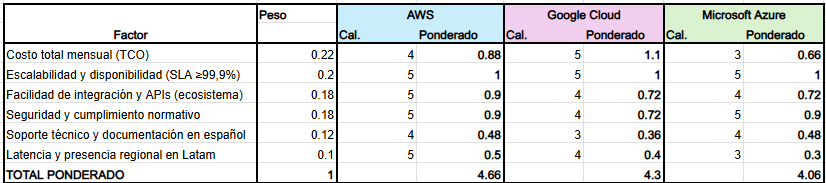
\includegraphics[width=0.8\textwidth]{img/Estudio_Tecnico_img-014.png}
\caption{Datos de alternativas para pasarelas de pago}
\end{figure}

\begin{table}[H]
\centering
\begin{tabular}{p{3cm}p{2cm}p{2cm}p{2cm}p{2cm}p{2cm}p{2cm}}
\toprule
\textbf{Alternativa} & \textbf{Costo TCO (22\%)} & \textbf{Escalabilidad (20\%)} & \textbf{Integración (18\%)} & \textbf{Seguridad (18\%)} & \textbf{Soporte (12\%)} & \textbf{Total} \\
\midrule
Amazon Web Services & 4 & 5 & 5 & 4 & 4 & 4.48 \\
Microsoft Azure & 3 & 4 & 4 & 5 & 3 & 3.82 \\
Google Cloud Platform & 3 & 4 & 4 & 4 & 3 & 3.64 \\
\bottomrule
\end{tabular}
\caption{Matriz de decisión (infraestructura cloud)}
\end{table}

Decisión seleccionada: Amazon Web Services (AWS). Obtuvo el puntaje más alto y se selecciona como la infraestructura cloud para el proyecto por su ecosistema de integración que permite conectar la plataforma con servicios como PayU, Twilio SendGrid y Truora. Su arquitectura con Amazon EC2, Auto Scaling y balanceadores de carga garantiza más de 99,99\% de disponibilidad y soporte técnico en español 24/7.

\subsectiontitle{2.2.3 Base de datos}

Comparamos las tres tecnologías más robustas del mercado: PostgreSQL, MongoDB y MySQL.

La selección se basó en cinco factores determinantes para el proyecto en Colombia.

\begin{table}[H]
\centering
\begin{tabular}{p{3cm}p{5cm}p{2cm}p{5cm}}
\toprule
\textbf{Factor} & \textbf{Descripción} & \textbf{Peso} & \textbf{Justificación} \\
\midrule
Escalabilidad y flexibilidad & Capacidad de crecimiento y soporte de esquemas de datos variables. & 25\% & Los itinerarios de viaje requieren una base de datos que se adapte a cambios constantes sin migraciones complejas. \\
\addlinespace
Rendimiento y latencia & Velocidad de respuesta en operaciones de consulta y escritura. & 20\% & La experiencia del usuario depende de la rapidez al consultar disponibilidad de servicios turísticos en tiempo real. \\
\addlinespace
Costo total (TCO) & Gastos asociados a licencias, infraestructura y mantenimiento. & 15\% & Es vital optimizar el presupuesto utilizando herramientas de código abierto con alta eficiencia operativa. \\
\addlinespace
Facilidad de integración & Compatibilidad con el stack tecnológico (Java/Spring Boot). & 20\% & El uso de microservicios demanda tecnologías con drivers maduros y soporte nativo para agilizar el desarrollo. \\
\addlinespace
Seguridad y cumplimiento & Protocolos de cifrado y alineación con normativas legales. & 20\% & Es obligatorio cumplir con la Ley 1581 de 2012 para la protección de datos personales de los viajeros en Colombia. \\
\bottomrule
\end{tabular}
\caption{Factores detallados del componente Base de datos}
\end{table}

Realizamos el análisis de alternativas de cada una como se muestra en la imagen con la matriz de decisión.

\begin{figure}[H]
\centering
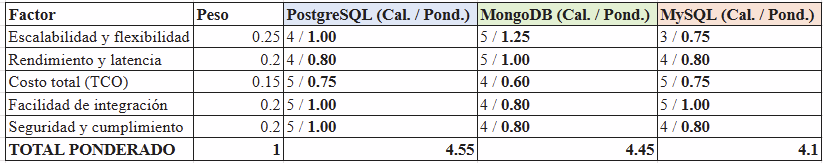
\includegraphics[width=0.8\textwidth]{img/Estudio_Tecnico_img-019.png}
\caption{Matriz de decisión para base de datos}
\end{figure}

\begin{table}[H]
\centering
\footnotesize
\begin{tabular}{p{2cm}p{2cm}p{2cm}p{2cm}p{2cm}p{2cm}p{2cm}}
\toprule
\textbf{Alternativa} & \textbf{Escalabilidad (25\%)} & \textbf{Rendimiento (20\%)} & \textbf{Costo (15\%)} & \textbf{Integración (20\%)} & \textbf{Seguridad (20\%)} & \textbf{Total} \\
\midrule
PostgreSQL & 4 & 4 & 5 & 5 & 5 & 4.45 \\
MongoDB & 5 & 4 & 4 & 4 & 4 & 4.20 \\
MySQL & 3 & 4 & 5 & 5 & 4 & 4.05 \\
\bottomrule
\end{tabular}
\caption{Matriz de decisión (Base de datos)}
\end{table}

Luego de aplicar la matriz de ponderación obtuvimos que PostgreSQL es la mejor opción como el motor de base de datos, pues su puntaje final es superior al de los demás, destacándose por su equilibrio entre la seguridad transaccional necesaria para procesar reservas y la flexibilidad requerida.

\subsectiontitle{2.2.4 Pasarela de pagos}

Los factores para tener en cuenta para este componente son:

\begin{table}[H]
\centering
\begin{tabular}{p{3cm}p{5cm}p{2cm}p{5cm}}
\toprule
\textbf{FACTOR} & \textbf{DESCRIPCIÓN} & \textbf{PESO (\%)} & \textbf{JUSTIFICACIÓN} \\
\midrule
Seguridad y certificaciones & Nivel de protección de datos y cumplimiento de estándares de seguridad (SSL/TLS, PCI DSS, antifraude). & 30\% & Es fundamental para proteger la información financiera de los usuarios, prevenir fraudes y generar confianza en la plataforma de reservas. \\
\addlinespace
Costo por transacción & Comisión que cobra la pasarela por cada pago procesado (porcentaje o tarifa fija). & 25\% & Influye directamente en los costos operativos del proyecto y en el margen de rentabilidad de la plataforma, especialmente cuando el volumen de transacciones es alto. \\
\addlinespace
Velocidad de procesamiento del pago & Tiempo que tarda la plataforma en confirmar una transacción desde que el usuario realiza el pago. & 20\% & Es importante porque una confirmación rápida mejora la experiencia del usuario, reduce la probabilidad de abandono de la compra y permite confirmar reservas en tiempo real dentro de la plataforma. \\
\addlinespace
Compatibilidad de métodos de pago & Cantidad de medios de pago que acepta la pasarela (tarjetas, PSE, billeteras digitales, etc.). & 15\% & Permite ofrecer mayor flexibilidad a los usuarios al momento de pagar, aumentando la probabilidad de completar la reserva y adaptándose a diferentes preferencias de pago. \\
\addlinespace
Facilidad de integración con la aplicación & Nivel de complejidad técnica para integrar la pasarela con la plataforma mediante APIs o SDK. & 10\% & Una integración sencilla reduce el tiempo de desarrollo, facilita el mantenimiento del sistema y permite implementar el servicio de pagos de forma más eficiente. \\
\bottomrule
\end{tabular}
\caption{Factores detallados del componente pasarela de pagos}
\end{table}

A continuación, se procederá con la recolección de los datos de cada alternativa y se realizará la calificación de las tres alternativas de pasarelas de pago.

\begin{table}[H]
\centering
\footnotesize
\begin{tabular}{p{2cm}p{2cm}p{2.5cm}p{2.5cm}p{2cm}p{2cm}}
\toprule
\textbf{Alternativa} & \textbf{Velocidad} & \textbf{Costo} & \textbf{Seguridad} & \textbf{Métodos} & \textbf{Integración} \\
\midrule
Wompi & $\sim$2 seg & 2.65\% + \$700 & PCI DSS, SSL/TLS & Tarjetas, PSE, Nequi & API REST \\
\addlinespace
PayU & $\sim$3 seg & 3.29\% + \$300 & PCI DSS, SSL/TLS & Tarjetas, PSE, efectivo & API completa \\
\addlinespace
Mercado Pago & $\sim$2 seg & 3.29\% + \$800 & PCI DSS, SSL/TLS & Tarjetas, PSE, billetera & API REST \\
\bottomrule
\end{tabular}
\caption{Datos por factor para cada alternativa (pasarelas de pago)}
\end{table}

\begin{table}[H]
\centering
\footnotesize
\begin{tabular}{p{2cm}p{2cm}p{2cm}p{2cm}p{2cm}p{2cm}p{2cm}}
\toprule
\textbf{Alternativa} & \textbf{Velocidad (20\%)} & \textbf{Costo (25\%)} & \textbf{Seguridad (30\%)} & \textbf{Métodos (15\%)} & \textbf{Integración (10\%)} & \textbf{Total} \\
\midrule
Wompi & 4 & 4 & 5 & 5 & 4 & 4.45 \\
PayU & 3 & 3 & 5 & 5 & 4 & 4.00 \\
Mercado Pago & 4 & 2 & 5 & 4 & 5 & 3.90 \\
\bottomrule
\end{tabular}
\caption{Matriz de decisión (pasarelas de pago)}
\end{table}

Tras aplicar la matriz de decisión ponderada, la pasarela de pagos Wompi obtuvo la mayor puntuación. Este resultado indica que Wompi presenta el mejor desempeño global según los factores evaluados. Por lo tanto, se selecciona como la alternativa más adecuada para la implementación de la pasarela de pagos en la plataforma.

\subsectiontitle{2.2.5 Integración con proveedores turísticos}

Los factores para tener en cuenta para este componente son:

\begin{table}[H]
\centering
\begin{tabular}{p{3cm}p{5cm}p{2cm}p{5cm}}
\toprule
\textbf{FACTOR} & \textbf{DESCRIPCIÓN} & \textbf{PESO (\%)} & \textbf{JUSTIFICACIÓN} \\
\midrule
Cobertura de destinos & Número de países y proveedores (aerolíneas, hoteles, tours) disponibles a través de la plataforma & 35\% & Determina la oferta que el usuario verá. \\
\addlinespace
Costo de integración & Costo total del setup, mantenimiento y tarifas por uso (COP/mes) & 15\% & Importante para controlar el presupuesto del proyecto \\
\addlinespace
Disponibilidad de datos & Latencia de respuesta (ms) & 25\% & Datos actualizados y rápidos son esenciales para reservas confiables. \\
\addlinespace
Confiabilidad & Porcentaje de uptime garantizado por SLA, estabilidad de la API & 25\% & Un sistema confiable evita fallas en reservas y errores en la app. \\
\bottomrule
\end{tabular}
\caption{Factores detallados del componente de integración con proveedores turísticos}
\end{table}

A continuación, se procederá con la recolección de los datos de cada alternativa y se realizará la calificación de las tres alternativas para la integración proveedores turísticos.

\begin{table}[H]
\centering
\begin{tabular}{p{2.5cm}p{2cm}p{2cm}p{2cm}p{2cm}p{2cm}}
\toprule
\textbf{Alternativa} & \textbf{Cobertura de destinos (35\%)} & \textbf{Costo de integración (15\%)} & \textbf{Disponibilidad de datos (25\%)} & \textbf{Confiabilidad (25\%)} & \textbf{Total} \\
\midrule
Amadeus & 5 & 3 & 5 & 5 & 4.70 \\
Sabre & 5 & 3 & 5 & 5 & 4.70 \\
APIs directas & 2 & 4 & 3 & 3 & 2.80 \\
\bottomrule
\end{tabular}
\caption{Matriz de decisión (integración con proveedores turísticos)}
\end{table}

Tras aplicar la matriz de decisión ponderada, tanto Amadeus como Sabre mostraron resultados similares en los criterios medibles. La elección de Amadeus se fundamenta en su mayor facilidad de uso y rapidez de implementación, así como en su presencia consolidada en el mercado latinoamericano.

\sectiontitle{BIBLIOGRAFÍA}

\begin{itemize}
    \item Wompi. (2024). Documentación para desarrolladores y tarifas. Recuperado de https://docs.wompi.co
    \item Mercado Pago. (2024). Tarifas y medios de pago disponibles para comercios. Recuperado de https://www.mercadopago.com.co
    \item PayU. (2024). Guía de integración y costos de procesamiento de pagos. Recuperado de https://developers.payulatam.com
    \item PCI Security Standards Council. (2023). PCI DSS Quick Guide: Understanding the Payment Card Industry Data Security Standard. Recuperado de https://www.pcisecuritystandards.org
    \item Superintendencia Financiera de Colombia. (2023). Lineamientos sobre sistemas de pago electrónicos en Colombia. Recuperado de https://www.superfinanciera.gov.co
    \item Metrocuadrado. (2025). Arriendo oficina en Bogotá, Quinta Camacho (3 baños). https://www.metrocuadrado.com/inmueble/arriendo-oficina-bogota-quinta-camacho-3-banos/532-M3112386
    \item Amazon Web Services. (2025). Amazon EC2 On-Demand Instance Pricing. Amazon Web Services. https://aws.amazon.com/ec2/pricing/on-demand/
    \item Amazon Web Services. (2025). Amazon RDS Pricing. Amazon Web Services. https://aws.amazon.com/rds/pricing/
    \item Amazon Web Services. (2025). Amazon RDS for PostgreSQL Pricing. Amazon Web Services. https://aws.amazon.com/rds/postgresql/pricing/
    \item Amazon Web Services. (2025). Amazon RDS for MySQL Pricing. Amazon Web Services. https://aws.amazon.com/rds/mysql/pricing/
    \item Amazon Web Services. (2025). Amazon API Gateway Pricing. Amazon Web Services. https://aws.amazon.com/api-gateway/pricing/
    \item Amazon Web Services. (2025). Amazon S3 Pricing. Amazon Web Services. https://aws.amazon.com/s3/pricing/
    \item Amazon Web Services. (2025). AWS Lambda Pricing. Amazon Web Services. https://aws.amazon.com/lambda/pricing/
    \item Amazon Web Services. (2025). Amazon OpenSearch Service Pricing. Amazon Web Services. https://aws.amazon.com/opensearch-service/pricing/
    \item Amazon Web Services. (2025). Amazon SQS Pricing. Amazon Web Services. https://aws.amazon.com/sqs/pricing/
    \item Amazon Web Services. (2025). Amazon SNS Pricing. Amazon Web Services. https://aws.amazon.com/sns/pricing/
    \item Amazon Web Services. (2025). Amazon ElastiCache Pricing. Amazon Web Services. https://aws.amazon.com/elasticache/pricing/
    \item Amazon Web Services. (2025). AWS Pricing Calculator. Amazon Web Services. https://calculator.aws/
    \item Amazon Web Services. (2025). What is AWS?. Amazon Web Services. https://aws.amazon.com/what-is-aws/
    \item Amazon Web Services. (2025). Amazon EC2 T3 Instances. Amazon Web Services. https://aws.amazon.com/ec2/instance-types/t3/
    \item Amazon Web Services. (2025). Amazon EC2 Auto Scaling. Amazon Web Services. https://aws.amazon.com/autoscaling/
    \item Amazon Web Services. (2025). Amazon EC2 Multi-AZ Deployments. Amazon Web Services. https://aws.amazon.com/rds/features/multi-az/
    \item Amazon Web Services. (2025). AWS Key Management Service (KMS). Amazon Web Services. https://aws.amazon.com/kms/
    \item Amazon Web Services. (2025). AWS Global Infrastructure: Regions and Availability Zones. Amazon Web Services. https://aws.amazon.com/about-aws/global-infrastructure/regions\_az/
    \item Amazon Web Services. (2025). AWS Marketplace. Amazon Web Services. https://aws.amazon.com/marketplace/
    \item Freshworks. (2025). Freshdesk Pricing Plans. Freshworks. https://www.freshworks.com/freshdesk/pricing/
    \item Featurebase. (2025). Zendesk Pricing 2025: Is It Worth It?. Featurebase Blog. https://www.featurebase.app/blog/zendesk-pricing
    \item Algolia. (2025). Algolia Pricing. Algolia. https://www.algolia.com/pricing
    \item CheckThat AI. (2026). Algolia Pricing 2026: Plans, Costs \& Real Examples. CheckThat AI. https://checkthat.ai/brands/algolia/pricing
    \item Ptolemay. (2025). Best AI Search Engines for Mobile Apps in 2025. Ptolemay Blog. https://www.ptolemay.com/post/best-in-app-ai-search-2025-algolia-vs-openai-vs-elasticsearch
    \item dolarhoy.co. (2026). Precio del dólar en Colombia — TRM 5 de abril de 2026. dolarhoy.co. https://www.dolarhoy.co/
\end{itemize}

\end{document}
